\section{\acrshort{das} and Digital Signal Processing Techniques}
\label{back:dsp}

\subsection{Distributed Acoustic Sensing Data}
\label{back:das}

\acrshort{das} data can be interpreted as a multi-sensor time series, where each channel (sensor) stores signal values for different sample times. THis data can be stored in different file formats, but due to the hierarchical nature of the data, formats such as TDMS \cite{10.1145/800196.805973} or \acrshort{hdf5} \cite{koranne2011hierarchical} are commonly used \cite{spica2022pubdas}. Their hierarchical nature is ideal for complex datasets, which often require additional metadata. Regardless of the chosen format, certain metadata are crucial for effectively handling and interpreting these data, including:
\begin{itemize}
    \item \textbf{Gauge length} is the spatial resolution of measurements.
    \item \textbf{Channel distance} stores information on spatial sampling. Not all channels along the total measurement are stored, so to understand the location of a signal, the gauge length, combined with the channel distance, tells us the exact distance from the start of the measurement.
    \item \textbf{Sample Rate}, or sample frequency, is the temporal resolution of the data and is measured in hertz. 
\end{itemize}
%
The \textit{spatio-temporal} aspects of \acrshort{das} come from how the data is represented. This data can be represented as a one-channel image, as shown by the seismic heatmap in Figure \ref{fig:dasframe-ex}. 
%
\begin{figure}[!h]
    \centering
    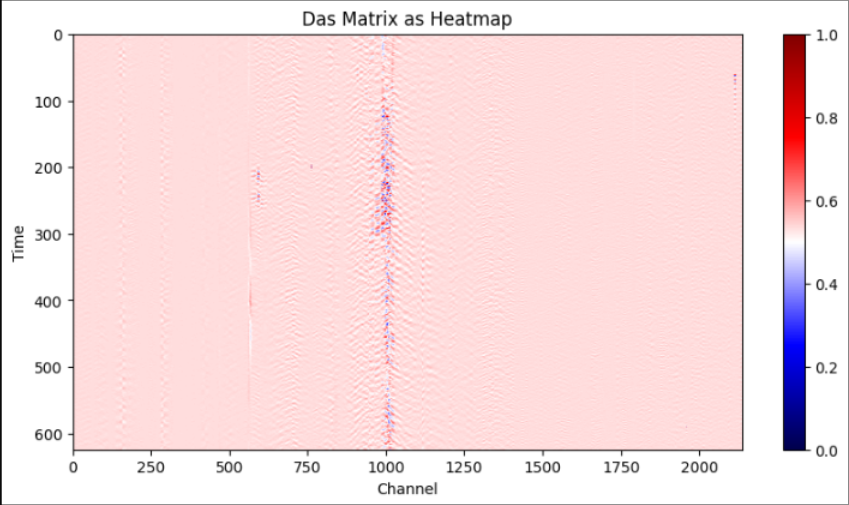
\includegraphics[width=0.7\linewidth]{figures/das_example.png}
    \caption{\textbf{Visualization} of normalized \acrshort{das} data as a heatmap. The vertical axis represents time (increasing downwards), while the horizontal axis shows a little more than 2000 spatial channels along the fiber. Color intensity indicates the strain rate, with reds representing higher rates and blues lower rates. The diagonal patterns in the middle likely represent propagating seismic waves or other dynamic strain events detected.}
    \label{fig:dasframe-ex}
\end{figure}
%
\subsubsection{Column- and Row-major Memory Alignment}
%
When working with large matrices, such as \acrshort{das} data, the order of the axis is important due to how different compilers access memory. When fetching a variable $x$, the \acrfull{cpu} will try to fetch a  \textit{cache-line}, and depending on the memory layout, this affects performance when iterating over the matrix. How a programming language or compiler organizes data in memory can significantly impact performance, especially for large-scale computations. The two types of memory alignment are \textit{column-major} and \textit{row-major} as shown in Figure \ref{fig:rowcol}.
%
\begin{figure}[!h]
    \centering
    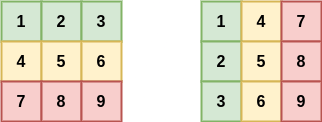
\includegraphics[width=0.5\linewidth]{figures/rowcol.png}
    \caption{Row-major (Left) and column-major (Right) memory ordering}
    \label{fig:rowcol}
\end{figure}
%
In the case of \acrshort{das} data, where calculations are often performed on a per-channel level, a language like Julia, MatLab, or Fortran would benefit from storing each channel in a column. This alignment can lead to several advantages, including:
\begin{enumerate}
\item \textbf{Improved cache utilization:} When processing data channel by channel, column-major storage ensures that the data for each channel is contiguous in memory, reducing cache misses.
\item \textbf{Reduced memory fragmentation:} Storing long time series for each channel in columns can lead to better memory allocation and less fragmentation.
\item \textbf{Vectorization opportunities:} Many modern processors support \acrfull{simd} operations, which can be more efficiently applied to contiguous data \cite{ren2006optimizing}.
\end{enumerate}
%
\subsection{Radio Frequency Filtering}
%
\acrfull{rf} filtering is of paramount importance in \acrshort{das} and \acrfull{dsp}. The signal quality can be improved by removing unnecessary noise from the data, and can decrease the overall of signal loss. In general, there are four types of filters, and can be defined as follows:
%
\begin{itemize}
    \item \textit{Band-pass filters} only allows frequencies between two cutoff frequencies $F_{low}$ and $F_{high}$
    \item \textit{Band-stop filters} stops frequencies between two cutoff frequencies $F_{low}$ and $F_{high}$
    \item \textit{Low-pass filters} only allows frequencies above the cut-off frequency $F_{low}$
    \item \textit{High-pass filters} only allows frequencies above the selected frequency $F_{high}$
\end{itemize}
%
A common approach to preprocessing \acrshort{das} data usually involves applying a bandpass to the signal matrix. Due to \acrshort{das} data being sensitive and capturing a broad range of frequencies, limiting the signals to a range of interest, depending on domain and application is beneficial.

\vspace{0.5cm}

\begin{figure}[!h]
    \centering
    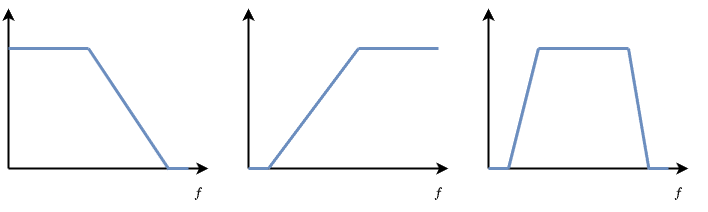
\includegraphics[width=0.8\linewidth]{figures/lowhighpass.png}
    \caption{Low-, High- and Band-pass filters}
    \label{fig:rffilters}
\end{figure}
%
\subsection{Tukey Window}
\label{dsp:tukey}

Window functions are functions often used in \acrshort{dsp} to avoid artifacts. This is done by setting values outside a pre-defined interval to zero and applying a taper from the passband to the first zero value. The Tukey window \cite{tukey1967introduction}, also known as the \textit{cosine-tapered window}, is a common approach to reducing edge effects, and can be formulated as such:

\[
    w(x)= 
\begin{cases}
    \frac{1 + \cos{2 \pi \alpha (x + \frac{1-\alpha}{2})}}{2}, & \text{if } x \leq \frac{1-\alpha}{2}\\
    1,              & \text{if } \frac{\alpha}{2} < x \leq \frac{\alpha}{2}\\
    \frac{1 + \cos{2 \pi \alpha (x - \frac{1-\alpha}{2})}}{2}, & \text{if } x > \frac{1-\alpha}{2}
\end{cases}
\]
where a higher $\alpha$ leads to a smoother cutoff in the output.
%\begin{figure}[!h]
%    \centering
%    \includegraphics[width=0.6\linewidth]{figures/tukey_windows_high_res.jpg}
%    \caption{Tukey window across different $\alpha$ values. The window becomes a rectangle when $\alpha = 0$}
%    \label{fig:tukeywindow}
%\end{figure}
\subsection{Resampling}
%
''Resampling methods are statistical procedures that reuse the sample data for the purpose of statistical inference''\cite{https://doi.org/10.1002/widm.1054}. In many applications, data is often initially collected at a very high sampling rate to capture fine details. However, this high sampling rate is not computationally efficient or even necessary for all analytical purposes. Down-sampling, also referred to as decimation within the \acrshort{dsp} field, is a form of resampling where the sampling rate is reduced, can be applied to:
%
\begin{itemize}
    \item Decrease memory consumption for data storage
    \item Reduce computational time for data processing
    \item Balance the trade-off between processing efficiency and data resolution
\end{itemize}
%
By reducing the sampling rate, one may retain the essential characteristics of the data while reducing data volume and computational requirements. However, one must be careful to avoid aliasing and ensure that the resampled data accurately represents the phenomena of interest. For \acrshort{das} data, this can differ drastically from one experiment to another. 
